% !TeX recipe = Tectonic
% CV - Marko Rosic - tailored for Deel, Lead Product Designer - Fintech
% Compile with: cd cv && tectonic Marko_Rosic_CV_deel_fintech.tex
\documentclass[a4paper,9.5pt]{article}

% ── Font ──────────────────────────────────────────────────────────────
\usepackage{fontspec}
\setmainfont{Fira Sans}[
  BoldFont       = {Fira Sans Bold},
  ItalicFont     = {Fira Sans Italic},
  BoldItalicFont = {Fira Sans Bold Italic}
]
\newfontfamily\symfont{Zapf Dingbats}

% ── Layout ────────────────────────────────────────────────────────────
\usepackage[a4paper, top=1.5cm, bottom=1.4cm, left=1.8cm, right=1.8cm]{geometry}
\usepackage{microtype}

% ── Colors ────────────────────────────────────────────────────────────
\usepackage{xcolor}
\definecolor{darktext}{HTML}{111111}
\definecolor{midgray}{HTML}{555555}
\definecolor{lightgray}{HTML}{999999}
\definecolor{hairline}{HTML}{BBBBBB}

% ── Links ─────────────────────────────────────────────────────────────
\usepackage[hidelinks]{hyperref}
\urlstyle{same}
\usepackage[normalem]{ulem}

% ── Lists ─────────────────────────────────────────────────────────────
\usepackage{enumitem}

% ── Tables ────────────────────────────────────────────────────────────
\usepackage{array}

% ── TikZ ──────────────────────────────────────────────────────────────
\usepackage{tikz}
\usetikzlibrary{calc}

% ── Section headings ──────────────────────────────────────────────────
\usepackage{titlesec}
\titleformat{\section}
  {\normalfont\small\bfseries}
  {}{0em}{\MakeUppercase}
  [\vspace{3pt}{\color{darktext}\hrule height 0.4pt}]
\titlespacing*{\section}{0pt}{22pt}{12pt}

% ── Page style ────────────────────────────────────────────────────────
\pagestyle{empty}
\setlength{\parindent}{0pt}
\setlength{\parskip}{0pt}

% ── Column dimensions ─────────────────────────────────────────────────
\newlength{\cvdatecol}  \setlength{\cvdatecol}{2.5cm}
\newlength{\cvsymcol}   \setlength{\cvsymcol}{1cm}
\newlength{\cvcontcol}  \setlength{\cvcontcol}{\dimexpr\textwidth-\cvdatecol-\cvsymcol\relax}

% ── Symbol counter ────────────────────────────────────────────────────
\newcounter{cvsymn}
\newif\ifcvfirst\cvfirsttrue

% ── TikZ asterisk with named remember-picture node ───────────────────
\newcommand{\cvastsym}{%
  \begin{tikzpicture}[remember picture, baseline=(sym-\thecvsymn.base)]
    \node[inner sep=0pt, outer sep=0pt, text=darktext, font=\normalsize\symfont] (sym-\thecvsymn) {✱};
  \end{tikzpicture}%
}

% ── Portfolio button ──────────────────────────────────────────────────
\newcommand{\portfoliobutton}{%
  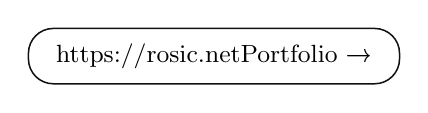
\begin{tikzpicture}[baseline=(btn.base)]
    \node[draw=darktext, rounded corners=9pt,
          inner xsep=10pt, inner ysep=5.5pt,
          line width=0.55pt, font=\small,
          outer sep=0pt] (btn)
      {\href{https://rosic.net}{Portfolio~→}};
  \end{tikzpicture}%
}

% ── Connector ─────────────────────────────────────────────────────────
\newdimen\cvyprev
\newdimen\cvycurr
\newcommand{\cvdrawconnect}{%
  \edef\prevn{\the\numexpr\value{cvsymn}-1\relax}%
  \begin{tikzpicture}[overlay, remember picture]
    \coordinate (cvprev) at (sym-\prevn.center);
    \coordinate (cvcurr) at (sym-\thecvsymn.center);
    \pgfextracty{\cvyprev}{\pgfpointanchor{cvprev}{center}}%
    \pgfextracty{\cvycurr}{\pgfpointanchor{cvcurr}{center}}%
    \ifdim\cvyprev>\cvycurr%
      \draw[line width=0.35pt, color=hairline]
        ($(sym-\prevn)+(0,-4.5pt)$) -- ($(sym-\thecvsymn)+(0,4.5pt)$);%
    \fi%
  \end{tikzpicture}%
}

% ── Entry macros ──────────────────────────────────────────────────────
\newcommand{\cventry}[3]{%
  \stepcounter{cvsymn}%
  \par\vspace{13pt}%
  \noindent%
  \makebox[\cvdatecol][r]{\small\bfseries\color{midgray}#1}%
  \makebox[\cvsymcol][c]{\cvastsym}%
  \parbox[t]{\cvcontcol}{%
    {\bfseries #2}\\[2.5pt]
    {\small#3}%
  }%
  \ifcvfirst\cvfirstfalse\else\cvdrawconnect\fi%
  \par%
}

\newcommand{\cventrynote}[4]{%
  \stepcounter{cvsymn}%
  \par\vspace{13pt}%
  \noindent%
  \makebox[\cvdatecol][r]{\small\bfseries\color{midgray}#1}%
  \makebox[\cvsymcol][c]{\cvastsym}%
  \parbox[t]{\cvcontcol}{%
    {\bfseries #2}\\[2.5pt]
    {\small#3}\\[2.5pt]
    {\footnotesize\itshape\color{lightgray}#4}%
  }%
  \ifcvfirst\cvfirstfalse\else\cvdrawconnect\fi%
  \par%
}

% ── Bullet list ───────────────────────────────────────────────────────
\newenvironment{cvitems}{%
  \vspace{1pt}%
  \begin{itemize}[
    leftmargin = \dimexpr\cvdatecol+\cvsymcol+0.55em\relax,
    label      = {•},
    topsep     = 4pt,
    itemsep    = 3pt,
    parsep     = 0pt,
    partopsep  = 0pt
  ]\small\interlinepenalty=10000%
}{\end{itemize}}

\newcommand{\skillblock}[2]{%
  {\small\bfseries #1}\newline%
  {\small\color{midgray}#2}%
}

% ══════════════════════════════════════════════════════════════════════
\begin{document}
% ══════════════════════════════════════════════════════════════════════

% ── HEADER ────────────────────────────────────────────────────────────
\vspace*{-0.3cm}
\noindent{\fontsize{30}{36}\selectfont\bfseries Marko Rosić}%
\hfill\makebox[0pt][r]{\portfoliobutton\hspace{2pt}}
\par\vspace{3pt}
{\small\color{midgray}%
  Cara Du\v{s}ana 118, Belgrade, Serbia~\textbar~%
  +381 60 585 44 55~\textbar~%
  \href{mailto:marko@rosic.net}{\uline{marko@rosic.net}}~\textbar~%
  \href{https://rosic.net}{\uline{rosic.net}}%
}

% ── SUMMARY ───────────────────────────────────────────────────────────
\section{Summary}

{\small Product designer and team lead with 15+ years on high-traffic,
multi-market consumer products. I build design systems that scale across
B2C and B2B surfaces, and I drive product decisions with research,
analytics, and A/B testing, cutting development time by 30\% and
time-to-market by 25\%. I design for real users who depend on the
product daily and I lead small teams by doing the work alongside them.
I use AI (including Claude Code) to prototype faster and to keep
improving how I and my team work.}

% ── EXPERIENCE ────────────────────────────────────────────────────────
\section{Experience}

\cventry{5/2025\,--\,Present}{Design Leadership Consultant}{%
  Beyond Clicks Studio (Independent) \textbar{} Belgrade, Serbia (Remote)}
\begin{cvitems}
  \item Senior design lead across several engagements, advising product
        and media companies on design systems, product strategy, and
        how design and engineering work together
  \item Lead multi-brand design-system and product UX for an
        international media group: token architecture, component
        conventions, accessibility, and handoff to engineering
  \item Lead AI\-orchestrated product and tooling work using Claude
        Code to build faster; designed and built an internal
        finance-and-operations product end to end as a case study
  \item Build working prototypes and Figma plugins to close the gap
        between design and what gets built
\end{cvitems}

\cventrynote{7/2024\,--\,5/2025}{Head of UX/UI}{%
  Gentoo Media \textbar{} Belgrade, Serbia}{%
  Gentoo Media was established following GiG Media's acquisition of
  Catena Media and subsequent spin-off of its media division.}
\begin{cvitems}
  \item Set design direction across multi-brand products through a
        company-wide design system
  \item Led a design team of seven, managing two team leads who each
        ran their own sub-team
  \item Changed how the team worked, cutting time-to-market for new
        features by 25\%
  \item Used analytics, A/B testing, and user feedback to drive
        product improvements
\end{cvitems}

\cventry{5/2021\,--\,7/2024}{Lead UX/UI Designer}{%
  Catena Media (acquired by GiG Media in 2023) \textbar{} Belgrade, Serbia}
\begin{cvitems}
  \item Directed UX from start to finish for high-traffic, multi-market
        consumer web products, using user-centred methods
  \item Built a design system for the flagship consumer product that
        cut development time by 30\%, and later ran it across 10+
        websites
  \item Ran A/B tests and used VWO and HotJar to measure and improve
        key flows
  \item Mentored junior designers and built a team that worked well
        together
\end{cvitems}

\cventry{10/2018\,--\,5/2021}{Senior UX/UI Designer}{%
  Catena Media \textbar{} Belgrade, Serbia}
\begin{cvitems}
  \item Led the redesign of the flagship consumer product, which raised
        mobile traffic by 20\% and user retention by 15\%
  \item Brought UX research into the product process and moved the team
        to decisions based on evidence
  \item Standardised UX practices across the product team
  \item Moved the team from Sketch to Figma, which improved how
        designers and engineers worked together
  \item Completed Catena Leadership Academy, an internal programme on
        cross-functional leadership and organisational management
\end{cvitems}

\cventry{12/2013\,--\,10/2018}{Interaction Designer}{%
  Smith Micro Software, Inc \textbar{} Belgrade, Serbia}
\begin{cvitems}
  \item Designed UX for carrier-branded Android apps shipped with
        Sprint and T-Mobile devices, including Visual Voicemail,
        Voicemail, and Sock Puppets
  \item Designed backend tooling for device management and an IoT
        location-based notification system, working across consumer
        interfaces and complex operational data views
  \item Worked closely with a graphic designer to deliver polished,
        on-brand interfaces across multiple carrier variants
\end{cvitems}

\cventry{2009\,--\,2013}{UI Designer}{%
  MySkin, Youngculture \textbar{} Belgrade, Serbia}
\begin{cvitems}
  \item Designed digital products and interfaces across client projects
        using user-centred methods
\end{cvitems}

\cventry{2005\,--\,2008}{Co-founder \& CEO}{%
  Mainstream d.o.o. \textbar{} Belgrade, Serbia}
\begin{cvitems}
  \item Co-founded a dial-up ISP; led operations, finance, and product
        design during the founding phase
\end{cvitems}

\cventry{2000\,--\,2005}{Web Designer/Developer}{%
  Various companies \textbar{} Belgrade, Serbia}

% ── SKILLS ────────────────────────────────────────────────────────────
\section{Skills}

\vspace{2pt}
\noindent
\begin{minipage}[t]{0.475\textwidth}
  \skillblock{Design \& Research}{%
    Figma, Axure RP, HTML/JS prototyping,
    Design Systems, Component Libraries,
    Interaction Design, Visual Design,
    User Research \& Testing (UserZoom,
    Optimal Workshop, UXtweak, HotJar)}

  \vspace{12pt}
  \skillblock{Data \& Analytics}{%
    Google Analytics, VWO, HotJar,
    Usability Testing, A/B Testing}
\end{minipage}%
\hspace{0.05\textwidth}%
\begin{minipage}[t]{0.475\textwidth}
  \skillblock{Leadership}{%
    Team Mentoring \& Talent Development,
    Cross-functional Stakeholder Management,
    Design Ops, Roadmap Planning, Project
    Management (Jira, Asana, Linear, Notion)}

  \vspace{12pt}
  \skillblock{Technical}{%
    HTML/CSS, PHP, JavaScript,
    Figma Plugin Development,
    MVP/POC Prototyping,
    Dev Complexity Assessment,
    AI-orchestrated delivery (Claude Code)}
\end{minipage}

% ── LANGUAGES ─────────────────────────────────────────────────────────
\section{Languages}

\begin{itemize}[leftmargin=1.2em, label={•},
    topsep=0pt, itemsep=2pt, parsep=0pt]
  \item {\small\textbf{English:} Fluent (Business Proficiency)}
  \item {\small\textbf{French:} Intermediate}
\end{itemize}

% ── EDUCATION ─────────────────────────────────────────────────────────
\section{Education}

\noindent{\small\bfseries Bachelor of Economics}\\[1pt]
{\small\color{midgray}Faculty for Business Studies,
Megatrend University, Belgrade \hfill 2002\,--\,2008}

\vspace{6pt}

\noindent{\small\bfseries Industrial Design Technician}\\[1pt]
{\small\color{midgray}School for Design, Belgrade
\hfill 1995\,--\,1999}
\begin{itemize}[leftmargin=1.2em, label={•},
    topsep=2pt, itemsep=0pt, parsep=0pt]
  \item {\small Established a foundation in design principles
        and aesthetics.}
\end{itemize}

\end{document}
